% !TeX root = ../main.tex

\chapter{系统测试与结果分析}

本章主要针对系统对仿真平台的仿真平台的需求,对整个仿真平台进行功能性和非功能性测试。
\section{仿真平台测试}

\subsection{测试环境}

因为公司项目的保密性,所有测试环节均在公司电脑上完成,测试电脑的配置如下所示:

CPU::Intel(R) Core(TM) i7-8700 CPU @3.2GHz

内存:32G

磁盘:1T

操作系统:Windows10

系统类型:64位操作系统

\subsection{测试工具和方法}

针对仿真平台,测试主要包括功能测试和非功能测试两个部分。功能测试主要从两个
方面进行测试,一方面,在整个平台构建之前,我们需要对建模好的各个硬件实例进行
功能测试,保证其功能正确。另一方面,在所有模块单独测试通过后,在整个仿真平台
构建时,我们从程序的输入输出为角度,对仿真平台的各个模块进行测试。这里主要对
硬件平台构建模块和仿真运行模块这两个模块的功能进行测试。针对仿真平台而言,我
们需要得到有效的仿真结果,包括时延、任务的开始结束信息、内存信息以及核的使用
情况等等。且仿真平台需要保证任务仿真执行时序与任务用例图的时序一致。

\subsection{硬件模块功能测试}
在对各个建模好的硬件模块进行功能测试主要测试的是实例化后的硬件模块时候能够
接收来自其他模块的消息并即时触发执行任务的流程、自身的硬件功能以及能够正常
与其他模块进行消息交互。在这个测试过程中,我们主要对GeneralFifo模块、Processor
模块以及Memory模块这三个模块进行测试。针对需求分析中对这三个模块提出的测试
指标进行测试,测试结果如表6.1、表6.2和表6.3所示:
\\
\begin{table}[]
    \centering
    \caption{GeneralFifo模块测试表}
    \begin{tabular}{|c|c|c|c|c|}
    \hline
    \textbf{序号} & \textbf{测试项}                                             & \textbf{操作流程}                                                                    & \textbf{预测结果}                                             & \textbf{实际结果} \\ \hline
    1           & \begin{tabular}[c]{@{}c@{}}能否正确的\\ 存取对象\end{tabular}     & \begin{tabular}[c]{@{}c@{}}调用GeneralFifo的方法\\ 函数来存取对象\end{tabular}               & \begin{tabular}[c]{@{}c@{}}通过调用函数方法\\ 成功存取对象\end{tabular} & 正确            \\ \hline
    2           & \begin{tabular}[c]{@{}c@{}}存取函数能否\\ 触发事件\end{tabular}    & \begin{tabular}[c]{@{}c@{}}调用该模块的事件接口\\ 去执行计数任务,存取对象后看\\ 每一步计数值是否正确\end{tabular} & 每一步计数值正确                                                  & 正确            \\ \hline
    3           & \begin{tabular}[c]{@{}c@{}}该模块外部\\ 接口方法是否正确\end{tabular} & \begin{tabular}[c]{@{}c@{}}通过存取对象,调用方法函数,\\ 观察结果是否正确\end{tabular}                & 结果正确                                                      & 正确            \\ \hline
    \end{tabular}
    \end{table}

如表6.1所示,我们对GeneralFifo模块进行了功能性测试,主要分为三个部分,测试项1
测试GeneralFifo模块作为一个先入先出队列的存取对象的功能,通过该模块提供的外部接口
方法,调用函数进行对象的存取,测试结果表示该功能正确。

测试项2测试GeneralFifo的事件机制是否能够被正确触发,GeneralFifo模块提供内部的event
事件接口,其他模块可以通过SimPy的yield机制去等待该event被触发。我们通过设置计数任务,
每次event被触发,计数任务被触发且打印计数值,我们通过像队列中存取对象来触发对象,
通过观察计数值,即可测试出GeneralFifo模块的事件机制是否正确。最后测试结果
表明GeneralFifo模块的事件机制正确。

测试项3测试GeneralFifo模块提供外部接口和方法是否正确,这部分我们只需通过调用
模块的外部接口即可测试,通过这部分测试表明GeneralFifo模块的外部接口正确。

\begin{table}[]
    \centering
    \caption{Processor模块测试表}
    \begin{tabular}{|c|c|c|c|c|}
    \hline
    \textbf{序号} & \textbf{测试项}                                                        & \textbf{操作流程}                                                                    & \textbf{预测结果}                                                    & \textbf{实际结果} \\ \hline
    1           & \begin{tabular}[c]{@{}c@{}}DSP模块处理能否\\ 即时并准确的\\ 接收任务实例\end{tabular} & \begin{tabular}[c]{@{}c@{}}向DSP模块入口Fifo发\\ 送任务实例,观察DSP模块\\ 对任务实例的解析\end{tabular} & \begin{tabular}[c]{@{}c@{}}DSP模块即时接\\ 收并正确解析\\ 任务实例\end{tabular} & 正确            \\ \hline
    2           & \begin{tabular}[c]{@{}c@{}}DSP任务处理时延\\ 是否与任务实例\\ 中一致\end{tabular}   & \begin{tabular}[c]{@{}c@{}}DSP接收并处理\\ 任务结束,查看\\ 仿真环境的时延\end{tabular}             & \begin{tabular}[c]{@{}c@{}}仿真环境的时延\\ 变化与任务实例\\ 中一致\end{tabular}  & 正确            \\ \hline
    3           & \begin{tabular}[c]{@{}c@{}}DMA模块处理能否\\ 即时并准确的\\ 接收任务实例\end{tabular} & \begin{tabular}[c]{@{}c@{}}向DMA模块入口Fifo发\\ 送任务实例,观察DMA模块\\ 对任务的解析\end{tabular}   & \begin{tabular}[c]{@{}c@{}}DMA模块即时接\\ 收并正确解析\\ 任务实例\end{tabular} & 正确            \\ \hline
    4           & \begin{tabular}[c]{@{}c@{}}DMA模块能否根据\\ 任务信息正确\\ 搬入搬出数据\end{tabular} & \begin{tabular}[c]{@{}c@{}}DMA执行完数据搬\\ 运任务,查看源地址与\\ 目的地址的内存变化\end{tabular}       & \begin{tabular}[c]{@{}c@{}}源地址与目的地址\\ 内存接收数据请求\end{tabular}      & 正确            \\ \hline
    5           & \begin{tabular}[c]{@{}c@{}}DMA模块与DSP\\ 模块能否流水\\ 线化执行任务\end{tabular} & \begin{tabular}[c]{@{}c@{}}向DMA模块发送任务实\\ 例观察整个任务能够\\ 完整执行\end{tabular}           & \begin{tabular}[c]{@{}c@{}}整个任务链完整\\ 且正确的执行\end{tabular}         & 正确            \\ \hline
    6           & \begin{tabular}[c]{@{}c@{}}HAC模块处理能否\\ 即时并准确的\\ 接收任务实例\end{tabular} & \begin{tabular}[c]{@{}c@{}}向HAC模块入口Fifo发\\ 送任务实例,观察HAC模块\\ 对任务实例的解析\end{tabular} & \begin{tabular}[c]{@{}c@{}}HAC模块即时接\\ 收并准确解析任\\ 务实例\end{tabular} & 正确            \\ \hline
    7           & \begin{tabular}[c]{@{}c@{}}HAC模块能否正\\ 确执行任务实例\end{tabular}          & \begin{tabular}[c]{@{}c@{}}HAC执行完整个任务实例\\ ,从对应HAC的日志中提\\ 取任务执行信息\end{tabular}    & \begin{tabular}[c]{@{}c@{}}任务执行信息与任\\ 务实例中信息一致\end{tabular}      & 正确            \\ \hline
    \end{tabular}
    \end{table}

如表6.2所示,我们对Processor模块的三种硬件模型进行了功能性测试。主要按照不同的硬件
模型分为三部分:

测试项1和测试项2主要测试DSP模块的硬件功能是否正确。测试项1通过构造测试用的任务实例,
并将测试用例发送到DSP模块的入口Fifo上,这部分测试当DSP模块的入口Fifo接收到任务实例
时,能不能立即处理任务实例,并能够正确的将任务实例中的任务信息解析出来;测试项2在
测试项1的基础上,测试了DSP模块处理任务实例,任务是否能够被正确执行,DSP任务只体
现时延的变化,只要保证在任务执行结束后,仿真环境的仿真时延变化与任务实例中信息一致
即可。从两项测试的结果来看,DSP模块的硬件功能符合要求。

测试项3\textasciitilde 5主要测试了DMA模块的硬件功能以及DMA模块和DSP模块流水线执行任务的能力。
测试项3通过构造测试用的任务实例,将测试用例发送到DMA模块的入口Fifo上,DMA模块
能够立即取出任务实例并正确的解析任务实例中的任务信息;测试项4在测试项3的基础上
对DMA模块对任务实例的处理能力进行测试,DMA模块负责数据的搬入搬出,我们只需要查看
源地址与目的地址对应的内存模块查看是否收到来自DMA的数据请求;测试项5是测试DMA模块
和DSP模块的流水线执行任务链的能力,在业务场景中常常会出现数据搬运后立即对数据进行
处理的场景,为了满足这种业务场景,测试项5通过构造带有数据搬运以及数据处理的任务链
级的任务实例,观察DMA模块执行完数据搬运能否通知目标DSP实例去执行数据处理任务。根据
测试结果显示,DMA模块的硬件功能以及DMA模块和DSP模块流水线执行任务的能力符合要求。

测试项6和测试项7主要测试HAC模块对任务的处理能力,测试项6通过构造在HAC模块上处理
的特定任务实例,HAC模块能能够立即接收任务实例并且正确的解析出任务实例中的任务信息;
测试项7通过查看对应HAC的日志去提取HAC模块在执行测试用例时的具体任务信息,通过任务
的执行信息,我们从时延变化、数据搬运等方面可以看出任务有没有正确执行。从两个测试项
的测试结果可以看出HAC模块对任务实例的处理能力符合要求。

\begin{table}[]
    \centering
    \caption{Memory模块测试表}
    \begin{tabular}{|c|c|c|c|c|}
    \hline
    \textbf{序号} & \textbf{测试项}                                                 & \textbf{操作流程}                                                          & \textbf{预测结果}                                                  & \textbf{实际结果} \\ \hline
    1           & \begin{tabular}[c]{@{}c@{}}能否正确的\\ 接收读写\\ 数据请求\end{tabular}  & \begin{tabular}[c]{@{}c@{}}发送读写数据请求\\ 到入口Fifo上,\\ 观察其解析结果\end{tabular} & \begin{tabular}[c]{@{}c@{}}解析结果\\ 正确\end{tabular}              & 正确            \\ \hline
    2           & \begin{tabular}[c]{@{}c@{}}能否正确的\\ 处理读写\\ 数据请求\end{tabular}  & \begin{tabular}[c]{@{}c@{}}查看对应模块日志文\\ 件中的数据处理信息\end{tabular}          & \begin{tabular}[c]{@{}c@{}}数据处理信息\\ 与数据请求中\\ 信息一致\end{tabular} & 一致            \\ \hline
    3           & \begin{tabular}[c]{@{}c@{}}能否与其他\\ 模块正确的\\ 消息交互\end{tabular} & \begin{tabular}[c]{@{}c@{}}查看处理完任\\ 务后,模块的\\ 返回信息\end{tabular}         & \begin{tabular}[c]{@{}c@{}}返回信息\\ 发送到对\\ 应模块\end{tabular}      & 正确            \\ \hline
    \end{tabular}
    \end{table}

如表6.3所示我们对Memory模块对数据请求的接收、处理以及消息交互的能力。测试项1
通过构造读写数据请求发送到Memory模块的入口Fifo上,Memory模块需要区分为读数据请求
以及写数据请求,再解析出数据处理的任务信息。测试结果表明Memory模块能够及时接收数据
请求并对数据请求进行正确解析。

测试项2在测试项1的基础上测试Memory模块对数据处理请求的执行能力。Memory模块在解析完
数据处理请求之后,需要根据请求的地址来将请求分为更小一级的Bank操作符,读写数据均按
照Bank级别进行操作,我们在对应Memory模块的日志文件中可以查看Bank读写操作的执行情况。
测试结果为数据处理请求的执行信息与数据处理请求所携带的任务信息一致,表明Memory模块
能正确执行数据处理请求。

测试项3测试Memory模块在数据处理结束后即时返回数据处理完成信息的能力。Memory模块在
完成数据处理请求之后,需向发送请求的模块返回请求完成的消息,我们只需查看消息内容以及
是否正确时间发送即可。测试结果表明Memory模块在请求完成之后返回的消息正确且返回消息
事件正确。

\subsection{硬件平台构建模块测试}

硬件平台构建模块的功能主要是解析硬件配置文件、实例化硬件模型以及构建硬件平台。
这三个功能将硬件配置文件中的硬件平台有关信息解析出来实例化硬件模型,并通过总
线模块将各个模型连接起来构建成为一个完整的硬件平台。硬件平台构建模块的测试结
果如表6.4所示:

\begin{table}[]
    \centering\small
    \caption{硬件平台构建模块测试表}
    \begin{tabular}{|c|c|c|c|c|}
    \hline
    \textbf{序号} & \textbf{测试项}                                               & \textbf{操作流程}                                                                & \textbf{预期结果}                                          & \textbf{实际结果} \\ \hline
    1           & \begin{tabular}[c]{@{}c@{}}是否能够解析硬件配\\ 置文件的信息\end{tabular} & 运行Task类中Load函数                                                               & \begin{tabular}[c]{@{}c@{}}硬件配置信息\\ 包含在类里\end{tabular} & 正确            \\ \hline
    2           & \begin{tabular}[c]{@{}c@{}}能否正确实例化硬\\ 件模型\end{tabular}     & \begin{tabular}[c]{@{}c@{}}运行PlatformBuilder类中\\ init函数\end{tabular}         & \begin{tabular}[c]{@{}c@{}}所有模型类\\ 成功创建\end{tabular}   & 正确            \\ \hline
    3           & \begin{tabular}[c]{@{}c@{}}能否正确构建硬件\\ 平台\end{tabular}      & \begin{tabular}[c]{@{}c@{}}运行SaeSimulator类中\\ build\_platform函数\end{tabular} & \begin{tabular}[c]{@{}c@{}}平台正确\\ 构建\end{tabular}      & 正确            \\ \hline
    \end{tabular}
    \end{table}

如表6.4所示我们对硬件平台构建模块进行了测试,测试项1通过运行PlatformBuilder类中
Load函数对硬件配置文件进行解析,我们可以调试过程中在类中找到所有硬件配置信息,
通过验证所有信息均已解析。

测试项2通过运行PlatformBuilder类中init函数根据测试1项中解析并保存的配置信息
将硬件平台中的所有硬件模型一一实例化,我们会通过对实例化的模型与硬件配置文件中
的模型类型与个数进行对比,来判断是否所有模型均已正确实例化。

测试项3中通过运行SaeSimulator类中的build\_platform函数将测试项2中实例化的所有
硬件模块根据硬件配置文件中的路由信息连接起来,构建形成完整的仿真平台。仿真平台的
功能实现主要通过后续仿真运行结果来进行测试,仿真平台的构建过程的输出信息如图6-1
所示:

\begin{figure}
    \centering
    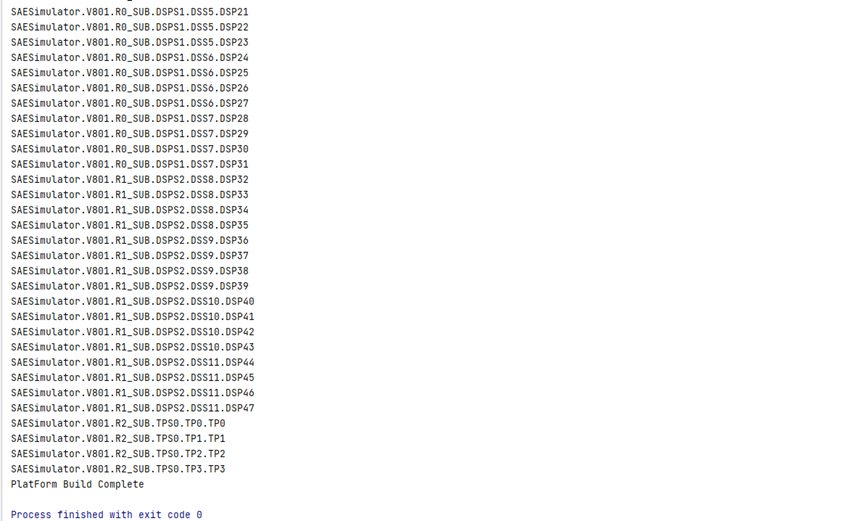
\includegraphics[width=1\textwidth]{硬件平台构建输出消息.png}
    \caption{硬件平台构建输出消息}
    \label{fig:badge}
\end{figure}

\subsection{仿真平台运行模块测试}

仿真平台运行模块功能主要要保证输入的任务用例能够正确的解析任务图信息、调度模块能够按照任务执行
顺序正确读取任务、仿真平台能够将整个任务图按序执行完毕。这些功能将任务图中信息解析出来并由调度
模块读取分配执行,使整个任务用例在仿真平台上完整的运行完毕。同时我们也需要保证任务执行时序以及
关键信息的准确性。仿真平台运行模块的测试结果如表6.5所示:

\begin{table}[]
    \centering\normalsize
    \caption{仿真平台运行模块测试表}
    \begin{tabular}{|c|c|c|c|c|}
    \hline
    \textbf{序号} & \textbf{测试项}                                               & \textbf{操作流程}                                                      & \textbf{预期结果}                                            & \textbf{实际结果} \\ \hline
    1           & \begin{tabular}[c]{@{}c@{}}是否能够完整解析任\\ 务图信息\end{tabular}   & \begin{tabular}[c]{@{}c@{}}运行TaskGraphMgnt\\ 类中Load函数\end{tabular} & \begin{tabular}[c]{@{}c@{}}任务图信息完整包\\ 含在类中\end{tabular}  & 正确            \\ \hline
    3           & \begin{tabular}[c]{@{}c@{}}DMA模块能否正\\ 确执行任务\end{tabular}   & \begin{tabular}[c]{@{}c@{}}发送DMA任务到\\ 硬件模块上执行\end{tabular}         & \begin{tabular}[c]{@{}c@{}}数据能够正确搬\\ 运到相应位置\end{tabular} & 正确            \\ \hline
    4           & \begin{tabular}[c]{@{}c@{}}DSP模块能否正确\\ 执行任务\end{tabular}   & \begin{tabular}[c]{@{}c@{}}发送DSP任务到\\ 硬件模块上执行\end{tabular}         & \begin{tabular}[c]{@{}c@{}}任务执行时延与\\ 任务信息一致\end{tabular} & 正确            \\ \hline
    5           & \begin{tabular}[c]{@{}c@{}}HAC模块能否正确\\ 执行任务\end{tabular}   & \begin{tabular}[c]{@{}c@{}}发送HAC任务到\\ 硬件模块上执行\end{tabular}         & \begin{tabular}[c]{@{}c@{}}任务执行结果与\\ 任务信息一致\end{tabular} & 正确            \\ \hline
    6           & \begin{tabular}[c]{@{}c@{}}仿真平台能否完整\\ 运行整个任务图\end{tabular} & \begin{tabular}[c]{@{}c@{}}运行主函数中的\\ SimRun函数\end{tabular}         & \begin{tabular}[c]{@{}c@{}}任务图中所有任\\ 务正确执行\end{tabular}  & 正确            \\ \hline
    7           & \begin{tabular}[c]{@{}c@{}}仿真运行结果时序\\ 是否正确\end{tabular}    & \begin{tabular}[c]{@{}c@{}}对比数据库仿真信\\ 息与任务用例信息\end{tabular}        & 两者信息一致                                                   & 正确            \\ \hline
    \end{tabular}
    \end{table}

如表6.5我们对仿真平台仿真运行模块进行了测试,测试项1通过运行TaskGraphMgnt模块的Load函数
去解析输入的用例文件。最后在调试过程中检测任务图信息是否完整包含在一个Graph类中,通过对比
用例中的任务信息以及测试过程中提取出来的Graph类中的信息,两者一致。任务图信息均包含在Graph
类中。

测试3\textasciitilde 5是为了测试各个硬件模块的功能是否正确。我们通过手动构造各种类型的任务用例到硬件模块的接口FIFO上来模拟调度器模块分配任务的流程,看各个硬件模块能不能正确执行任务用例,且任务执行结果是否和任务描述是否一致。测试结果显示各个硬件模块均能正确执行调度器分配的任务。

测试项6通过运行项目主函数中的SimRun函数运行仿真,函数参数包括任务用例名、任务图执行次数、输出数据库位置、Log文件是否记录等等。我们在硬件平台搭建完成的基础上,使用任务用例输入执行仿真,仿真运行输出信息如图6-2所示。且在数据库中将任务执行信息与任务用例中任务信息相对比,执行时序正确无误。

\begin{figure}
    \centering
    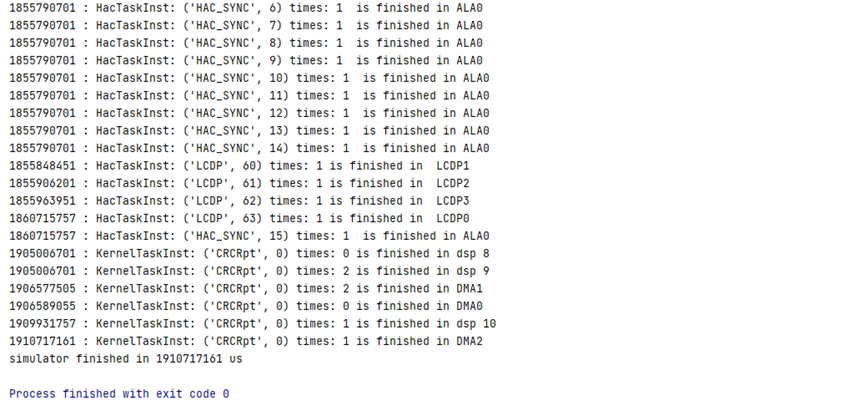
\includegraphics[width=1\textwidth]{仿真运行输出消息.png}
    \caption{仿真运行输出消息}
    \label{fig:badge}
\end{figure}

由上面两个方面的验证能够保证仿真平台的功能的正确性。能够满足业务需求以及后续设计空间探索的需求。

\subsection{仿真平台性能测试}
在对仿真平台功能方面进行测试的同时,我们需要对仿真平台的性能方面进行测试。我们在需求分析阶段提出了几个对于
仿真平台以及设计空间探索流程的性能测试指标,我们针对需求分析中表3-2中指标进行测试,测试结果如
表6.6所示:

\begin{table}[htb]
    \centering\normalsize
    \caption{仿真平台性能测试表}
    \begin{tabular}{|c|c|c|c|l}
    \cline{1-4}
    序号 & 测试项            & 预期结果              & 测试平均结果   &  \\ \cline{1-4}
    1  & 仿真硬件平台搭建时间     & \textless{}=5s    & 4.76s  &  \\ \cline{1-4}
    2  & 单次单小区仿真执行时间    & \textless{}=150s   & 135.6s &  \\ \cline{1-4}
    3  & 仿真结果时序是否与用例一致  & True              & True   &  \\ \cline{1-4}
    4  & 设计空间探索结果是否全局最优 & True              & True   &  \\ \cline{1-4}
    \end{tabular}
    \end{table}

如表6.3所示,通过对仿真平台以及设计空间探索流程进行多次运行,得到的测试结果如上表所示。
由测试结果可以看出仿真平台的单次单小区的执行时间低于预期值且远远低于原有SAE仿真平台的
单次单小区的执行时间,满足后续设计空间探索流程的需求。

在测试项3测试时,我们针对任务用例中的任务执行触发关系以及任务处理时间进行分析,通过读取
数据库文件中每个任务的执行时间以及任务的上下级任务进行分析,最终得到测试结果,任务均可以
在对应任务的触发以及相应条件下正确执行,仿真结果时序正确。

对于测试项4而言,在5.5.3节我们对设计空间探索的结果进行了详细的分
析,结果满足全局最优。针对需求分析阶段提出的性能需求的几大指标而言,测试结果都满足性能
测试指标需求。

\section{本章小结}

本章主要对仿真平台做了功能上的测试,仿真平台能够正确的构建硬件平台,并能够在硬件平台上运行任务用例,保证任务仿真的时序正确。同时也对设计空间探索的结果进行了分析,并得到了一些结论和在所有目标值方面比较优秀的设计方案。